% CHAPTER 1
\chapter{Introduction}
\label{chp:b1}

In recent years, deep neural networks have shown impressive performance in many vision related tasks such as image classification~\cite{he2015deep}, object detection~\cite{redmon2018yolov3} and image segmentation~\cite{long2015fully}. However, they are found to be vulnerable to intentionally crafted small perturbations called adversarial perturbations~\cite{szegedy2013intriguing}. These small perturbations added to the input image successfully change the output of a trained classifier by altering the logits large enough to change its decision to a preferred class~\cite{goodfellow2014explaining}. While these perturbations are optimized in \(\mathcal{L}_p\) spaces~\cite{carlini2017towards}, they are visible to human observers, since small \(\mathcal{L}_p\) does not always correspond to small visible perturbations~\cite{jordan2019quantifying,engstrom2018rotation}.
There is an ongoing research on finding difference metrics over 2D images that aligns with human visual perception, which is challenging due to the nature and lack of knowledge about the human vision. Multimedia compression standards have been developed to compress visual multimedia such as images and videos to reduce the amount of data with minimum amount of distortion to the perceived output. One of the most fundamental ideas of visual multimedia compression is that human vision is much less sensitive to the information loss in color than the luminance.
%evolution%
This observation is utilized in image compression as a technique known as ``chroma subsampling''. There are variants of chroma subsampling that only subsamples chrominance along horizontal axis (4:2:2) or both horizontal and vertical axes (4:2:0). Without further compression, (4:2:0) chroma subsampling reduces the size of an image effectively to half of its original size. Replacing the chroma components of the pixels in by neighboring chroma components does not yield visible artifacts. We employ this observation to derive a new type of adversarial attack based on spatial transformations in chroma channels of perceptual colorspaces. We apply spatial transformation only to the chroma components of input image while keeping the luminance component intact. Figure~\ref{fig:flowtochannels} shows the effect of a randomly initialized flow field applied to the luminance, chrominance and both set of channels. It is clear that spatial transformation in luminance channels causes visible distortions while chrominance only spatial transformations cause very subtle changes for human vision. This effect is much more highlighted when only the differences are observed after applying a flow field. Figure \ref{fig:outofgamut} shows the absolute pixel difference from the initial image when the same flow field is applied to RGB, \(C_{b}C_{r}\) and a*b* channels, respectively.
\begin{figure}[t]
    \centering
    \begin{subfigure}[b]{.30\linewidth}
        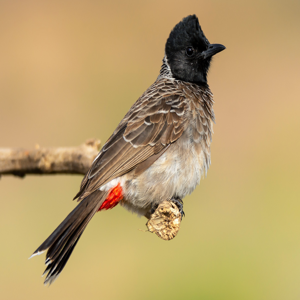
\includegraphics[width=\linewidth]{img.png}
        %        \caption{Original}
        \caption{}
    \end{subfigure}
    \begin{subfigure}[b]{.30\linewidth}
        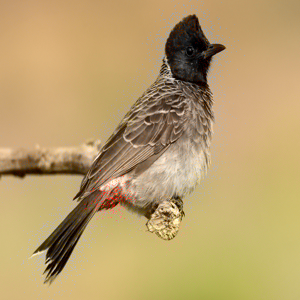
\includegraphics[width=\linewidth]{flowed_cbcr.png}
        %        \caption{Flow to CbCr channels}
        \caption{}
    \end{subfigure}
    \begin{subfigure}[b]{.30\linewidth}
        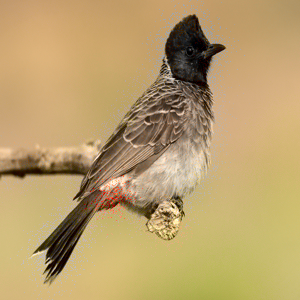
\includegraphics[width=\linewidth]{flowed_ab.png}
        %       \caption{Flow to \(a^*b^*\) channels}
        \caption{}
    \end{subfigure}
    \begin{subfigure}[b]{.30\linewidth}
        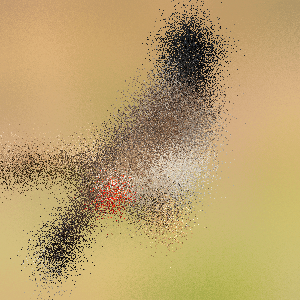
\includegraphics[width=\linewidth]{flowed_rgb.png}
        %      \caption{Flow to RGB channels}
        \caption{}
    \end{subfigure}
    \begin{subfigure}[b]{.30\linewidth}
        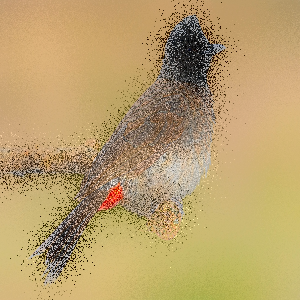
\includegraphics[width=\linewidth]{flowed_y.png}
        %     \caption{Flow to Y channel}
        \caption{}
    \end{subfigure}
    \begin{subfigure}[b]{.30\linewidth}
        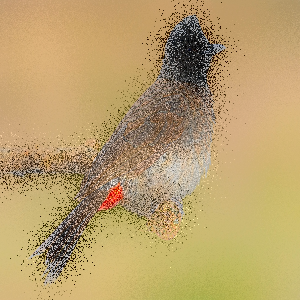
\includegraphics[width=\linewidth]{flowed_l.png}
        %\caption{Flow to L channel}
        \caption{}
    \end{subfigure}
    \caption{Effect of flow field applied to different channels, (a) original image, Images where flow field is applied to (b) \(C_{b}C_{r}\), (c) \(a^*b^*\), (d) RGB, (e) Y and (f) L channel. The magnitude of the flow is scaled up to emphasize the effect for illustration.}\label{fig:flowtochannels}
\end{figure}

\begin{figure}[t]
    \centering
    \begin{subfigure}[b]{.23\linewidth}
        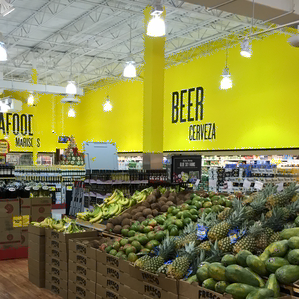
\includegraphics[width=\linewidth]{diff/209_lab_adv.png}
        \caption{}
    \end{subfigure}
    \begin{subfigure}[b]{.23\linewidth}
        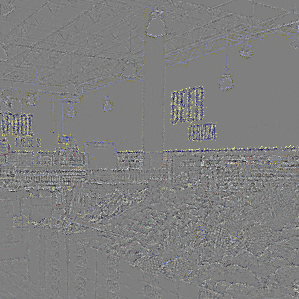
\includegraphics[width=\linewidth]{diff/209_rgb_diff.png}
        \caption{}
    \end{subfigure}
    \begin{subfigure}[b]{.23\linewidth}
        
\includegraphics[width=\linewidth]{diff/209_ycbcr_diff.png}
        \caption{}
    \end{subfigure}
    \begin{subfigure}[b]{.23\linewidth}
        
\includegraphics[width=\linewidth]{diff/209_lab_diff.png}
        \caption{}
    \end{subfigure}
    \caption{Visual difference from flow field applied to different channels, (a) original image, Visualization of pixel differences where flow field is applied to (b) RGB, (c) \(C_{b}C_{r}\), (d) \(a^*b^*\) channels. The magnitude of the flow is scaled up and contrast of the pixel differences is increased to increase the visibility for illustration. }\label{fig:diff}
\end{figure}

\begin{figure*}[t]
    \centering
    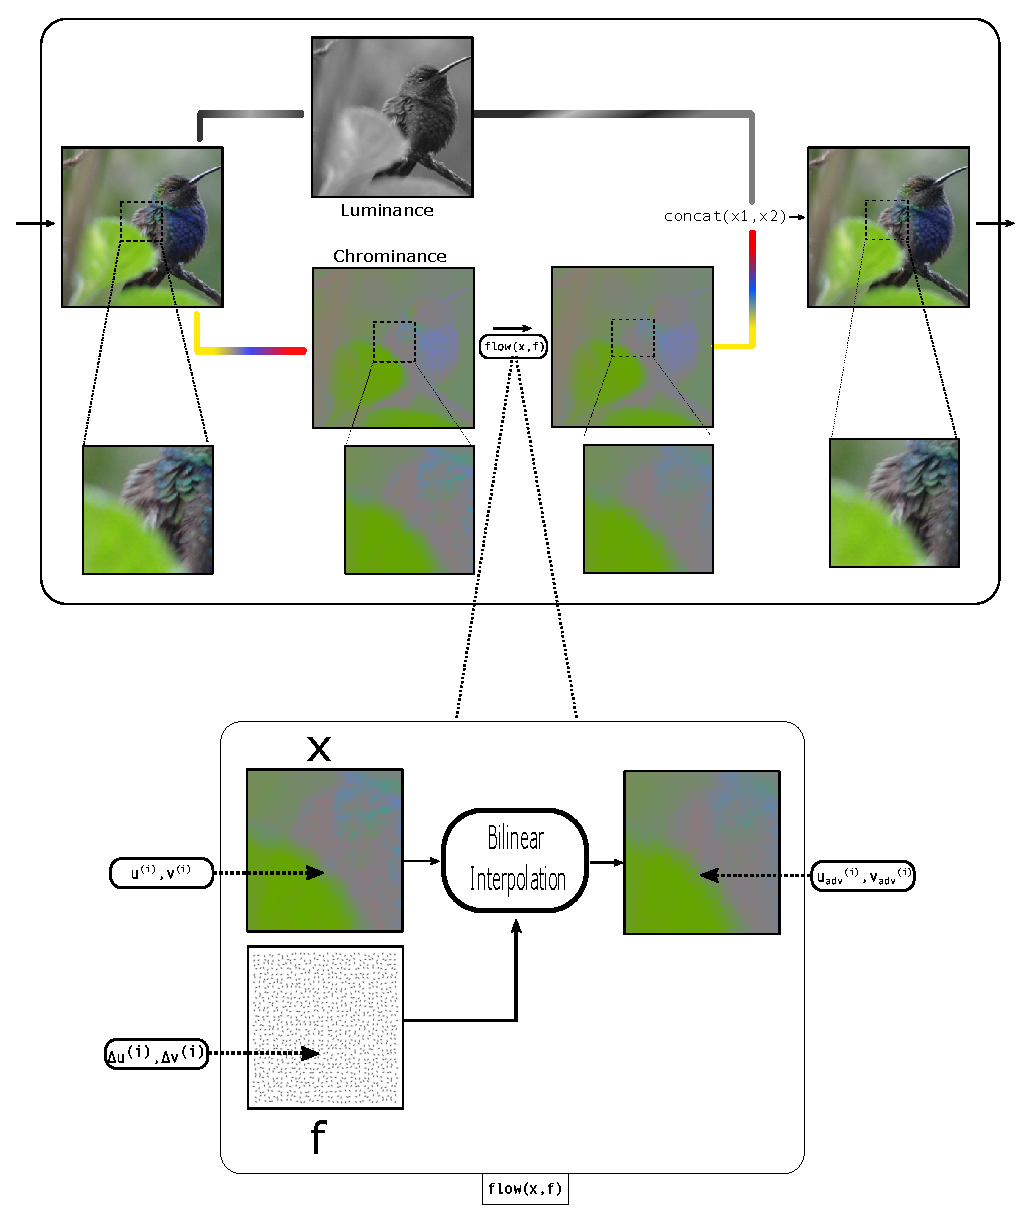
\includegraphics[width=0.8\linewidth]{illustration/drawing.eps}
    \caption{Visual illustration of the proposed adversarial example generation method. Luminance and chrominance channels are Y and \(C_{b}C_{r}\) when \(YC_{b}C_{r}\) colorspace and L and \(a^*b^*\) when CIELAB colorspace is used. Visual representation of flow field, subpixel restriction by \(\tanh\) and conversion of concatenated image back to RGB colorspace is omitted for brevity.}\label{fig:algorithm}
\end{figure*}
Lorem ipsum dolor sit amet, mea sanctus appetere id, ut blandit referrentur mel. Qui legendos mediocrem ei, mazim soluta praesent sed ut. Eam diam putent invidunt id. Cu his virtute interpretaris, quod latine at per. Has ex aliquip expetendis, per at duis suscipiantur, vix id laudem nostro omnesque. Te pro nusquam detracto, ius at fuisset disputando, cibo malorum dignissim ut pri.

Detracto definitiones mediocritatem at mel, eos te aeque delenit deseruisse. Sint volumus duo ei, sed petentium adolescens no. Agam facilisi dignissim ex vis. Vel te graece aperiam volumus. Te nec nulla noster inciderint, ridens labore pertinax cu ius, meis fugit movet pri ut. At probo docendi referrentur sit, quem magna nominavi nam cu. Nec ut eripuit vocibus, his ignota antiopam no.

Ipsum error suscipit an mei, has in pertinax repudiandae delicatissimi, vivendo patrioque est in. Et vix ignota maiestatis complectitur, mei adolescens percipitur et. Id eum dicit soleat, no animal impedit antiopam sit. Cu illud mucius eos, tempor delenit instructior nec eu.

Per et blandit patrioque, ubique incorrupte sit an, pro porro laoreet et. Mel blandit officiis disputando ea, eu pri sonet debitis appellantur. Cu numquam nominati temporibus mei, convenire efficiantur et nec. Mea et quando labores laoreet, ad sed utinam labitur perfecto. Mei appetere detraxit vituperata ea, quo discere epicurei ad, est novum doctus inciderint ad. His ne mucius labores, in vis quod ullum. Vidisse fabulas senserit sea id, ad usu mentitum consulatu, ocurreret deterruisset vel ne.

At euismod eruditi theophrastus est, sit te doctus molestiae. Ne natum elitr ullamcorper est. Cu malorum recusabo mei, ei mea laoreet reprimique. Persius discere nusquam mel ei, at inimicus posidonium sed. Vel ad unum illud \cite{Cohen1992}.

\section{Research Questions}

\section{Contributions of the Study}

\section{Organization of the Thesis}

